\documentclass[a4paper,12pt]{ctexart}
\usepackage{amsmath}
\usepackage{color}
\usepackage[top=25mm,bottom=25mm,left=20mm,right=20mm]{geometry}
\usepackage{graphicx}
\usepackage{pdfpages}% 直接插入pdf的宏包
\usepackage[colorlinks,linkcolor=red]{hyperref}
\renewcommand\thefigure{\thesection.\arabic{figure}}
\usepackage[superscript]{cite}
\bibliographystyle{unsrt}
\numberwithin{equation}{section}
\graphicspath{{pictures/}}
\author{李玉轩}
\title{Vortex中的Majorana零能摸}
\begin{document}
\maketitle
%
\includepdf{cover/cover.pdf}
%\newpage
%\tableofcontents
\section{文档说明}
本手册用来记录在重复论文中遇到的问题,以及计算程序编写过程中,物理公式与程序语言之间的转换关系。本文档所有的代码均已上传至\href{https://github.com/yxli8023/BdG}{GitHub},在使用代码之前,请先阅读\textbf{ReadMe}文件,其中亦有作者的邮箱,欢迎讨论。
\section{模型建立}
代码是用来重复\href{https://github.com/yxli8023/BdG/blob/master/article/PhysRevB.96.184508.pdf}{Vortex pinning by the point potential in topological superconductors:A scheme for braiding Majorana bound states}中的数值结果,其中主要的模型内容如下所示:
\begin{equation}
H = H_t+H_{SO}+H_{SC}
\end{equation}
\begin{equation}
H_t = -\sum_{<ij>}t_0\Phi_{ij}(c_{i\sigma}^\dagger c_{j\sigma}+H.c)+\sum_{i\sigma}(\sigma h-\mu)c_{i\sigma}^\dagger c_{i\sigma}+\sum_\sigma V_ic_{i_0\sigma}^\dagger c_{i_0\sigma}\label{eqhop}
\end{equation}
\begin{equation}
H_{SO}=\sum_{i}(i\lambda\Phi_{ij} c_{i\uparrow}^\dagger c_{i+\hat{x}\downarrow}+i\lambda\Phi_{ij} c_{i\downarrow}^\dagger c_{i+\hat{x}\uparrow}+H.c.
+\lambda\Phi_{ij}c_{i\uparrow}^\dagger c_{i+\hat{y}\downarrow}
-\lambda\Phi_{ij}c_{i\downarrow}^\dagger c_{i+\hat{y}\uparrow}+H.c.)\label{eqsoc}
\end{equation}
\begin{equation}
H_{SC}=\sum_i(\Delta_{ii}c_{i\uparrow}^\dagger c_{i\downarrow}^\dagger+H.c.)
\end{equation}
\begin{equation}
\sum_j 
\left[
\begin{array}{cccc}
H_{ij\uparrow\uparrow}&H_{ij\uparrow\downarrow}&\Delta_{jj}&0\\
H_{ij\downarrow\uparrow}&H_{ij\downarrow\downarrow}&0&-\Delta\\
\Delta_{jj}^\star&0&-H_{ij\downarrow\downarrow}^\star&-H_{ij\downarrow\uparrow}^\star\\
0&-\Delta_{jj}^\star&-H_{ij\uparrow\downarrow}^\star&-H_{ij\uparrow\uparrow}^\star
\end{array}
\right] \Psi_j^\eta=E_\eta\Psi_j^\eta\label{eq:5}
\end{equation}

where  $\Psi_j^\eta=(u_{j\uparrow}^\eta,u_{j\downarrow}^\eta,v_{j\downarrow}^\eta,v_{j\uparrow}^\eta)^T$and$\Delta_{jj}=\frac{V}{2}\sum_\eta u_{j\uparrow}^\eta v_{j\downarrow}^\eta\tanh(\frac{E_\eta}{2K_BT})$
$\sigma$代表自旋取向,向上为1向下为-1,$t_0$代表电子在相邻格点跳跃((hopping)时的能量,$\lambda$代表相邻格点之间的自旋轨道耦合(SOC)强度,$\Delta$是每个格点上不同自旋取向电子的配对能,$\mu$是体系的化学势,求和中的i是格点位置索引,公式中的i代表虚数单位。

通过模型建立,可以得到关于哈密顿量的矩阵形式,模型求解的关键点在于如何通过一系列的公式,正确的写出哈密顿量的矩阵形式,即就是方程(\ref{eq:5})中的矩阵。
\subsection{分析}
\begin{equation}
H=\sum_i(c_{i\uparrow}^\dagger,c_{i\downarrow}^\dagger,c_{i\downarrow},c_{i\uparrow}) \left[
\begin{array}{cccc}
H_{ij\uparrow\uparrow}&H_{ij\uparrow\downarrow}&\Delta_{jj}&0\\
H_{ij\downarrow\uparrow}&H_{ij\downarrow\downarrow}&0&-\Delta\\
\Delta_{jj}^\star&0&-H_{ij\downarrow\downarrow}^\star&-H_{ij\downarrow\uparrow}^\star\\
0&-\Delta_{jj}^\star&-H_{ij\uparrow\downarrow}^\star&-H_{ij\uparrow\uparrow}^\star
\end{array}
\right](c_{i\uparrow},c_{i\downarrow},c_{i\downarrow}^\dagger,c_{i\uparrow}^\dagger)^T
\end{equation}\label{eq6}
\subsubsection{hopping项}
在模型求解过程中,主要是通过建立超导BdG方程,并且构建出其对应的哈密顿量的矩阵形式,对矩阵进行对角化之后,同时可以得到相应的本征值和本征矢量。从模型的建立来看,主要是通过紧束缚近似的离散晶格模型来构造哈密顿量,在紧束缚近似中,仅仅考虑了每个格点和相邻位置的跳跃和耦合,则可以明白\textbf{公式中的i和j仅仅代表的是最近邻格点位置(此处的ij代表的是格点的位置,先简单的认为是个一维的链,那么可以仅仅通过i来代表格点的位置)}.
\subsubsection{couple项}
couple项的分析与hopping项分析过程类似,唯一不同的一点是,相邻格点之间的耦合,涉及到的是不同自旋取向之间的耦合,它的每一项仍然都处于矩阵的非对角线上。
\subsubsection{pair项}
从超导配对项的表达式中可以看到,它涉及到时同一个点不同自旋取向之间的配对,所以通过对矩阵的分析可以得知,它的每一项也都处于矩阵的非对角线上。
\subsubsection{others}
在hopping项中,第二项比较特殊($\sum_{i\sigma}(\sigma h-\mu)c_{i\sigma}^\dagger c_{i\sigma}$),从下角标可以知道,这一项同样是处于矩阵的对角线上,只不过不同的自旋取向对应着不同的值。自旋向上$\sigma=1$,自旋向下$\sigma=-1$,h代表的是Zeeman场的大小。

\subsection{矩阵构建}
由方程(\ref{eq6})的形式可以知道,对于每一个格点i,上面都定义了四个算符,假设我们考虑的晶格大小是xn*yn,那么在构建哈密顿量矩阵的时候选择的基矢量就应该是一个4*xn*yn长度的向量,对应的哈密顿量矩阵形式就是(4*xn*yn,4*xn*yn)大小.通过分析过程可以得知对于hopping项($H_{ij\sigma\sigma}$),每个自旋取向$\sigma$对应的$H_{ij}$都是一个xn*yn的小方阵,通过上面的分析,将整个矩阵分解为16个小矩阵,每个小矩阵(方阵)维度都是xn*yn,不过该矩阵的大多数元素都是0,属于稀疏矩阵。在这里需要强调一点,这16个小的分块矩阵是根据将基矢选择为$C^\dagger=(c_\uparrow^\dagger,c_\downarrow^\dagger,c_\downarrow,c_\uparrow)$,在这里省略了每个格点位置的索引,其实这里的每一个算符都应该是有xn*yn个的.$C^\dagger$与$C$中的算符进行组合,共有16中可能,这就是16个小的分块矩阵的来源.
\textbf{这里同样可以不按照上面$C^\dagger$中算符的顺序进行排列,可以选择自己在构建矩阵时能理解或者觉得简单的方式,虽然这样会使得矩阵内相同位置上的值有所改变,但是不会改变最终的结果}.在方程(\ref{eq:5})中,波函数$\Psi$的形式已经得知(即格点位置与自旋之间的联系),且注意到,索引指标j代表了晶格点阵的大小(在小的分块矩阵中),j=xn*yn,前面已经将矩阵分解成了16个小矩阵,且其中又有4个都是零,则需要考虑填充的只有12个分块矩阵(有些算符的组合在现在这个问题中本就不会存在,所以它对应的位置就是0).
\subsection{hopping项}
\begin{figure}[h]
\centering
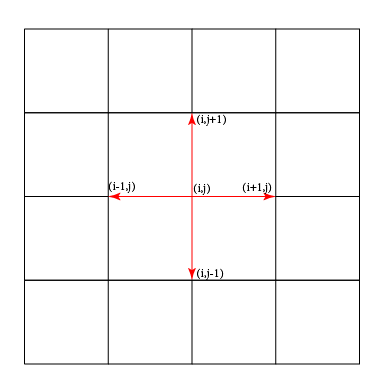
\includegraphics[scale=0.5]{SqLattice.png}
\caption{最近邻hopping}
\end{figure}\label{figHop}
hopping项中,不在对角线上的项是$c_{i\sigma}^\dagger c_{j\sigma}(i\neq j)$,紧束缚近似仅考虑最近邻的格点之间的行为,考虑二维正方点整,对于(i,j)格点上的电子,共有四个最近邻,如图\ref{figHop}所示.在这里所使用的均是二维点阵的索引,在进行矩阵的构建时,需要将这些二维的索引,转变成基矢中对应的索引.\textbf{举例说明:在(i,j)这个格点上,它所对应的$C^\dagger$中的产生算符的索引为(i-1)*xn + j,这里xn是正方格点在x方向的格点数,同样的yn是在y方向上的格点数.这个索引同样可以表示为(j-1)*yn + i,这就是如果将2维点阵上的点,映射成一维基矢上的换算方法,对于其它形式的算符,也是相同的转换技巧.这里还要说明一点,上面选取的是$C^\dagger$中的一个算符,它转换出来的索引,对应的是哈密顿量矩阵中的行索引,对于$C$中选取的算符,它转换出来的索引则对应的是哈密顿量矩阵中的列索引.}上面就是如何将一对算符(2个算符的组合)写成哈密顿量矩阵中的一个元素的方式,这样就可以初步对矩阵进行填值.在方程(\ref{eqhop})和(\ref{eqsoc})中可以看到,实空间的哈密顿量只是明确的写出了$c^\dagger c$的算符着形式,暂且称它是粒子的算符表示形式,但是由方程($\ref{eq6}$)可以看到,哈密顿量中同样还包括了$cc^\dagger$这种组合形式,称它为空穴,由于研究的是关于超导的问题,平均场近似下的哈密顿量是有粒子空穴对称性的,所以肯定会出现这种空穴型的算符,而上面所说的填值问题都是关于粒子的,并没有提及关于空穴该如何构建其哈密顿量对应的值.可以通过费米子算符的对易关系,将空穴的填值问题与粒子的填值联系到一起.
\begin{equation}
\{c^\dagger_i,c_j\}=c^\dagger_ic_j+c_jc^\dagger_i=0
\end{equation}
所以可以得到空穴和粒子的联系是
\begin{equation}
c_jc^\dagger_i=-(c_j^\dagger c_i)^\dagger
\end{equation}
所以只要知道了电子$c_j^\dagger c_i$的填值,将其共轭之后再添负号就是$c_jc_i^\dagger$的填值.再次强调,这里的ij是基矢的索引(也是矩阵元素的索引),而不是二维晶格的直角索引坐标,是它门的2维坐标转换成1维的基矢之后的索引.到这里就将哈密顿量中所有关于最近邻格点之间的项全部介绍完了,而剩下的不过是不同spin以及产生湮灭算符之间的组合,它们涉及到的是分块矩阵之间的组合,这个可以和最近邻矩阵元构建的过程相类比,就可以得到结果.
\subsection{Spin orbit couple 项}
从方程(\ref{eqsoc})中可以看到,它与hopping项(\ref{eqhop})唯一的区别就是此时产生算符和湮灭算符组合的时候,自旋是相反的.将隔着区别对应到矩阵中,从分块矩阵的角度上来讲,它门都是处于非对角线上的分块矩阵.如果以$C^\dagger=(c^\dagger_\uparrow,c^\dagger_\downarrow,c_\downarrow,c_\uparrow)$为基矢来构建矩阵的话,$c^\dagger_\uparrow c_\downarrow$对应的是(1,2)这个分块矩阵.
\begin{equation}
\left[
\begin{array}{cccc}
H_{ij\uparrow\uparrow}&\textcolor{red}{H_{ij\uparrow\downarrow}}&\Delta_{jj}&0\\
H_{ij\downarrow\uparrow}&H_{ij\downarrow\downarrow}&0&-\Delta_{jj}\\
\Delta_{jj}^\dagger&0&-H_{ij\downarrow\downarrow}^\dagger&-H_{ij\downarrow\uparrow}^\dagger\\
0&-\Delta_{jj}^\dagger&-H_{ij\uparrow\downarrow}^\dagger&-H_{ij\uparrow\uparrow}^\dagger
\end{array}
\right]\label{socm}
\end{equation}
其它项和这一项的构造方式完全相同,涉及到最近邻格点之间的问题时,处理方法与hopping项构造的方式也完全相同,是不过是hopping项对应的分块矩阵都是在方程(\ref{socm})的对角线上,而自旋轨道耦合项的分块矩阵则都是在副对角线上.
%---------------------------------------------------
\section{周期性边界问题}
\begin{figure}[ht]
\centering
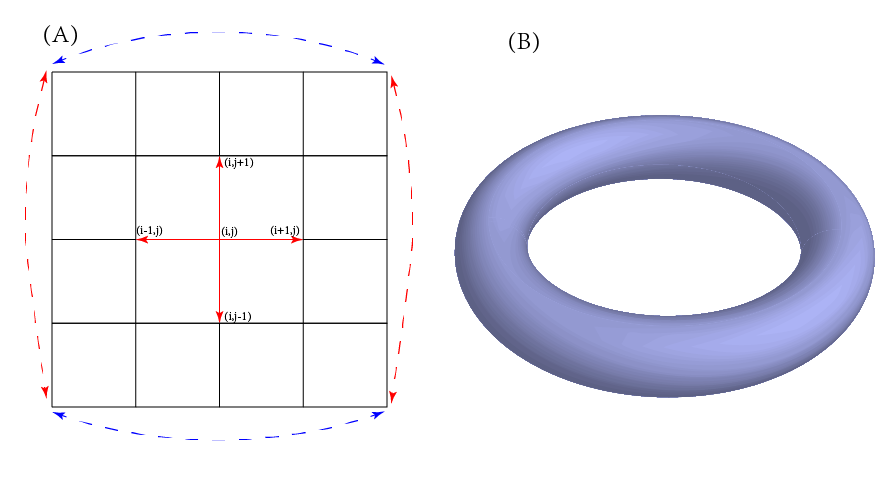
\includegraphics[scale=0.45]{periodic.png}
\caption{格点模型的周期边界条件}\label{per}
\end{figure}
在这个问题的处理过程之中,哈密顿量是从实空间中离散的格点上进行构建的,但是问题本身需要在实空间中去构造一个周期性边界条件的格点, 如图(\ref{per})所示,上边界和下边界连接到一起,左边界和右边界连接到一起,这样就可以形成一个环状结构,如图(\ref{per})(B)所示.然而要完成周期性边界构造的最主要的一点就是,对于这种$c_{i\sigma}^\dagger c_{j\sigma}$的构造算符组合(i,j代表基矢中的索引,j是i的最近邻),以二维点阵模型为例:最右边的格点,它右边的最近邻就是最左边的格点,最上边的格点它上边的最近邻就是和它同一列最下端的格点,如图(\ref{per})(A)中的连线所示,这就是在实空间构造周期性边界条件的方法.下面给出具体在程序中的实现:基矢为($c_{1\uparrow}^\dagger,\dots,c_{n\uparrow}^\dagger;c_{1\downarrow}^\dagger,\dots,c_{n\downarrow}^\dagger;c_{1\downarrow},\dots,c_{n\downarrow};c_{1\uparrow},\dots,c_{n\uparrow}$),$n=xn*yn,xn,yn$分别是x方向的格点数目和y方向的格点数目.第iy行最右边的格点索引为\textcolor{blue}{$(iy-1)*xn + xn$},该格点在周期边界条件下右边的最近邻位置是iy行第一个格点位置,其索引为\textcolor{blue}{(iy-1)*xn + 1};将上面的整个分析反过来既可以得到最左边格点位置上周期边界条件下左边的最近邻格点位置.下面考虑上下边界的周期性索引问题,第yn行,第ix个格点位置的索引为\textcolor{blue}{(yn-1)*xn + ix},它在周期性边界时上边的格点为第1行第ix个格点位置,其对应的索引为ix;同样的,上述过程反过来就是下边界到上边界的周期边界设置.上面就是如何在实空间中构建一个周期边界的方法.
\section{磁场位相设置}
\begin{figure}[ht]
\centering
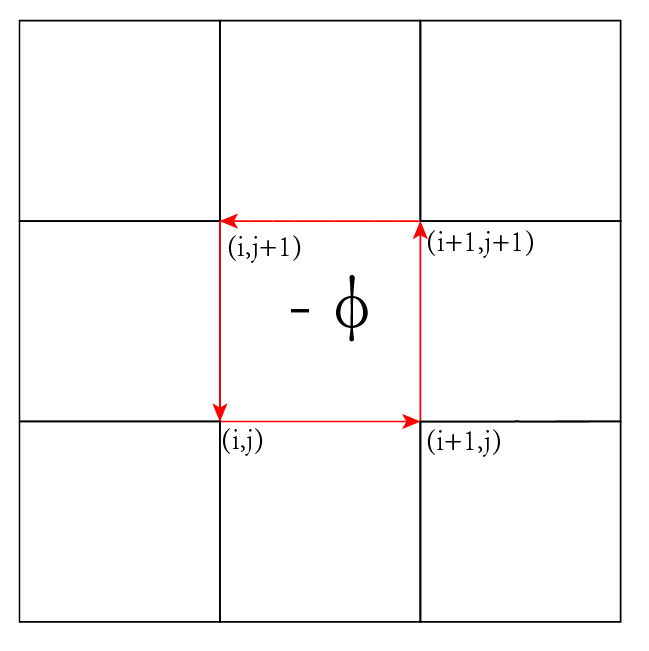
\includegraphics[scale=0.45]{flux2.png}
\caption{hopping位相设置}\label{magnet}
\end{figure}
在这个研究问题中,需要外加一个磁场,以次来产生vortex.磁场的选择采用朗道规范$\mathbf{A}=B_0(-y,0,0)$,其中$B_0$代表磁场大小.外加磁场之后,每一项涉及最近邻格点间的算符的组合形式,其对应前面的系数都要增加一个位相因子$$t_{i,j}=t^0_{i,j}e^{i\vec{A}(\vec{R_i}-\vec{R_j})}$$,其中$t^0_{i,j}$是未加入磁场时hopping的大小,这个增加位相的过程叫做\href{https://zhuanlan.zhihu.com/p/81170343}{派尔斯变换}.在这篇文章中,由于是在离散格点模型上讨论问题,磁场导致的额外位相是$exp[i\pi/\phi_0\int_{R_i}^{R_j}\vec{\mathbf{A}}(\mathbf{r})d\mathbf{r}]$,$\phi_0$是一个量子磁通,在这里取$\phi_0=\pi$.在二维点阵的构造下,只要使最近邻的项其位相变换后,在一个最小的循环内的位相剩余为$\phi_0$,那么在周期性边界条件下,一共会有$xn*yn$数量的小循环,如图(\ref{magnet})所示,最后所有小循环的位相累积为$2\phi_0$,系统的波函数与之前一样,即使得$\sum_{All (i,j)}$位相满足$exp[i\pi/\phi_0*2\phi_0]=1$,磁场振幅$B_0=2\pi/(xn*yn)$.

当不涉及到边界的时候,位相的设置方法如上所述;在碰到边界的时候,需要进行额外的一点考虑.在这里选择的朗道规范$\mathbf{A}=B_0(-y,0,0)$,由它的形式可以看到,y方向上的hopping并不会带有位相的变换,仅有x方向hopping才会涉及到位相的变换.\textcolor{red}{特意强调,这里的hopping不是单指哈密顿量中的hopping项,而是指所有的$c_i^\dagger c_j$项,即只要是不同格点之间算符的组合,就涉及到位相的变换,从哈密顿量中可以看到,自旋轨道耦合项同样存在这种形式的组合,所以它同样也要受到磁场的影响}.而y方向上唯一需要考虑位相的地方是在边界上.
\begin{figure}[ht]
\centering
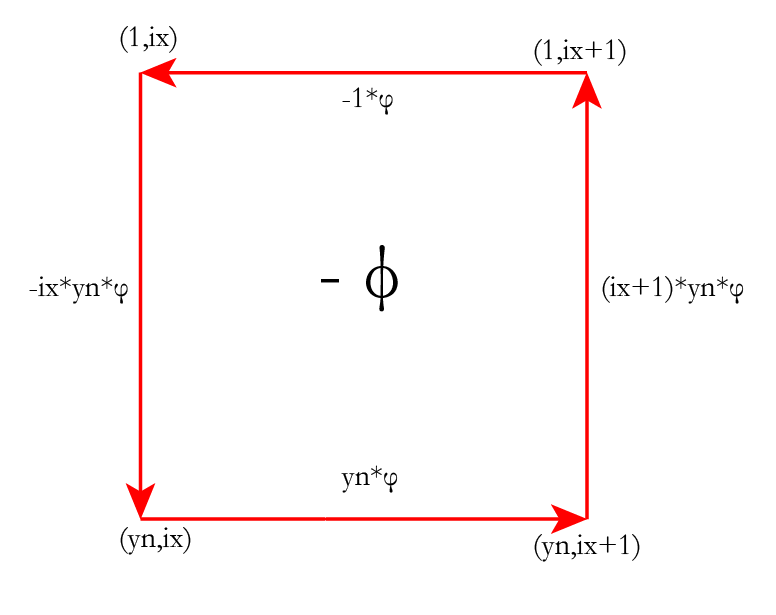
\includegraphics[scale=0.45]{flux1.png}
\caption{边界位相设置}\label{boundary}
\end{figure}
当由上边界跳跃到下边界的时候,在周期性边界的情况下,如果仅x方向存在位相变换,则形成的小循环并不能保证净胜位相是$\phi_0$(顺时针方向走一圈为$\phi_0$,逆时针方向走一圈则为$-\phi_0$),所以需要在边界上的y方向,从一个边界跳跃到另外一个边界的时候,额外的补充一个位相,使得整个循环的净胜位相是$\phi_0$,具体如何设置额外的位相,如图(\ref{boundary})所示.到此为止,所有关于文章计算所需要的技术细节都已展示完毕.
\section{矩阵对角化}
通过上面的内容将哈密顿量矩阵构建完成之后,剩下的工作就是将矩阵对角化,得到其对应的本征值和本征矢量,这里的矩阵对角化稍微提及一些.假设一个矩阵H,对他对角化的流程如下$$H=SDS^{-1}$$,其中D是一个对角矩阵,它的本一个对角线上的元素就对应着矩阵$H$的本征值,而$S$就是得到的本征矢量构成的矩阵,假设有一个本征矢为$E_n$,则矩阵$S$中的第$n$列就是这个本征值所对应的本征矢量.
\section{程序调试及检验}
下面列举几点程序编写技巧:1.文章中所求解的是一个哈密顿量,那么它的矩阵表示一定是个厄密矩阵,所以在执行矩阵对角化之前,首先检验一个矩阵是否是厄密的,因为如果取$xn=yn=48$,所对应的矩阵将会很大,矩阵对角化时间较长,提前对矩阵的验证可以避免由于矩阵构建错误,而浪费时间在对角化上;2.这是一个涉及到超导的问题,从哈密顿量的基矢上可以看到,通常将基矢写成南部(Nambu)表象的形式,即前半部分是产生算符,后半部分是湮灭算符,在这个问题中哈密顿量具有粒子空穴对称性,所以求解得到的本征值,一定是正负对称的$(E,-E)$同时出现,所以在矩阵是厄密的之后,可以通过对角化之后的本征值来判断是否矩阵构建是正确的;3.矩阵构建过程中,加入磁场后hopping项的位相改变是比较麻烦的,所以在构建矩阵时,对位相的赋值一定要特别仔细,否则容易导致矩阵构建出错,而这个位相的构建,在矩阵中并没有很好的技巧可以介绍,希望多加注意;4.超导的序参量是一个需要自洽求解的量,这一点在文章中已经明确提到,所以在第一次进行计算时,可以给超导序参量随便的一个值(也可以是每个格点都给随机值),然后进行自洽计算,这个随机值并不会对最后的结果有影响.
\section{最后}
大概拖了有大半年的时间,才终于将这个文档完全写完,主要是由于之前想把周期边界条件和位相的改变的东西,可以通过图的形式展现出来,最近正好学习了一些画图的软件,用它小试牛刀把之前剩下的工作都能给补充起来,也算是对前面自己所学知识的一个总结和理解.如果对文档中的内有不清楚或者不理解的,也欢迎通过邮箱联系.


\newpage
\includepdf[pages=2]{file/prb.pdf}	
\end{document}